% Created by tikzDevice version 0.10.1 on 2018-06-07 10:28:11
% !TEX encoding = UTF-8 Unicode
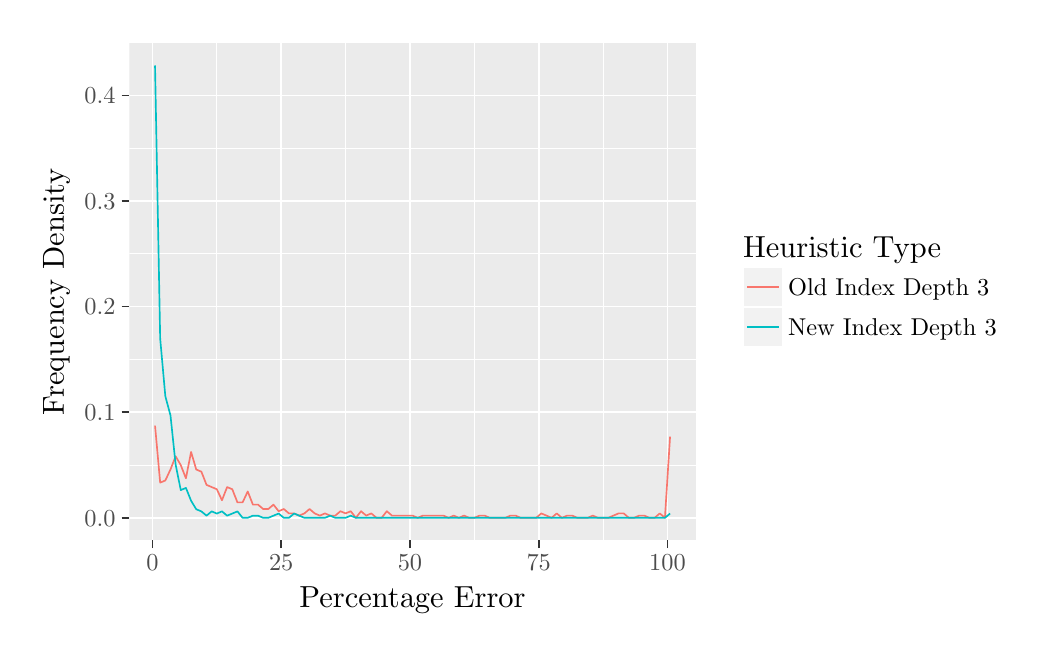
\begin{tikzpicture}[x=1pt,y=1pt]
\definecolor{fillColor}{RGB}{255,255,255}
\path[use as bounding box,fill=fillColor,fill opacity=0.00] (0,0) rectangle (361.35,216.81);
\begin{scope}
\path[clip] (  0.00,  0.00) rectangle (361.35,216.81);
\definecolor{drawColor}{RGB}{255,255,255}
\definecolor{fillColor}{RGB}{255,255,255}

\path[draw=drawColor,line width= 0.6pt,line join=round,line cap=round,fill=fillColor] (  0.00,  0.00) rectangle (361.35,216.81);
\end{scope}
\begin{scope}
\path[clip] ( 36.71, 31.53) rectangle (241.43,211.31);
\definecolor{fillColor}{gray}{0.92}

\path[fill=fillColor] ( 36.71, 31.53) rectangle (241.43,211.31);
\definecolor{drawColor}{RGB}{255,255,255}

\path[draw=drawColor,line width= 0.3pt,line join=round] ( 36.71, 58.78) --
	(241.43, 58.78);

\path[draw=drawColor,line width= 0.3pt,line join=round] ( 36.71, 96.94) --
	(241.43, 96.94);

\path[draw=drawColor,line width= 0.3pt,line join=round] ( 36.71,135.10) --
	(241.43,135.10);

\path[draw=drawColor,line width= 0.3pt,line join=round] ( 36.71,173.26) --
	(241.43,173.26);

\path[draw=drawColor,line width= 0.3pt,line join=round] ( 68.35, 31.53) --
	( 68.35,211.31);

\path[draw=drawColor,line width= 0.3pt,line join=round] (114.88, 31.53) --
	(114.88,211.31);

\path[draw=drawColor,line width= 0.3pt,line join=round] (161.41, 31.53) --
	(161.41,211.31);

\path[draw=drawColor,line width= 0.3pt,line join=round] (207.93, 31.53) --
	(207.93,211.31);

\path[draw=drawColor,line width= 0.6pt,line join=round] ( 36.71, 39.70) --
	(241.43, 39.70);

\path[draw=drawColor,line width= 0.6pt,line join=round] ( 36.71, 77.86) --
	(241.43, 77.86);

\path[draw=drawColor,line width= 0.6pt,line join=round] ( 36.71,116.02) --
	(241.43,116.02);

\path[draw=drawColor,line width= 0.6pt,line join=round] ( 36.71,154.18) --
	(241.43,154.18);

\path[draw=drawColor,line width= 0.6pt,line join=round] ( 36.71,192.35) --
	(241.43,192.35);

\path[draw=drawColor,line width= 0.6pt,line join=round] ( 45.09, 31.53) --
	( 45.09,211.31);

\path[draw=drawColor,line width= 0.6pt,line join=round] ( 91.61, 31.53) --
	( 91.61,211.31);

\path[draw=drawColor,line width= 0.6pt,line join=round] (138.14, 31.53) --
	(138.14,211.31);

\path[draw=drawColor,line width= 0.6pt,line join=round] (184.67, 31.53) --
	(184.67,211.31);

\path[draw=drawColor,line width= 0.6pt,line join=round] (231.20, 31.53) --
	(231.20,211.31);
\definecolor{drawColor}{RGB}{248,118,109}

\path[draw=drawColor,line width= 0.6pt,line join=round] ( 46.02, 73.02) --
	( 47.88, 52.40) --
	( 49.74, 53.19) --
	( 51.60, 57.16) --
	( 53.46, 61.92) --
	( 55.32, 58.74) --
	( 57.18, 53.98) --
	( 59.05, 63.50) --
	( 60.91, 57.16) --
	( 62.77, 56.36) --
	( 64.63, 51.60) --
	( 66.49, 50.81) --
	( 68.35, 50.02) --
	( 70.21, 46.05) --
	( 72.07, 50.81) --
	( 73.93, 50.02) --
	( 75.80, 45.26) --
	( 77.66, 45.26) --
	( 79.52, 49.22) --
	( 81.38, 44.46) --
	( 83.24, 44.46) --
	( 85.10, 42.88) --
	( 86.96, 42.88) --
	( 88.82, 44.46) --
	( 90.68, 42.08) --
	( 92.55, 42.88) --
	( 94.41, 41.29) --
	( 96.27, 41.29) --
	( 98.13, 40.50) --
	( 99.99, 41.29) --
	(101.85, 42.88) --
	(103.71, 41.29) --
	(105.57, 40.50) --
	(107.43, 41.29) --
	(109.30, 40.50) --
	(111.16, 40.50) --
	(113.02, 42.08) --
	(114.88, 41.29) --
	(116.74, 42.08) --
	(118.60, 39.70) --
	(120.46, 42.08) --
	(122.32, 40.50) --
	(124.18, 41.29) --
	(126.05, 39.70) --
	(127.91, 39.70) --
	(129.77, 42.08) --
	(131.63, 40.50) --
	(133.49, 40.50) --
	(135.35, 40.50) --
	(137.21, 40.50) --
	(139.07, 40.50) --
	(140.93, 39.70) --
	(142.80, 40.50) --
	(144.66, 40.50) --
	(146.52, 40.50) --
	(148.38, 40.50) --
	(150.24, 40.50) --
	(152.10, 39.70) --
	(153.96, 40.50) --
	(155.82, 39.70) --
	(157.68, 40.50) --
	(159.55, 39.70) --
	(161.41, 39.70) --
	(163.27, 40.50) --
	(165.13, 40.50) --
	(166.99, 39.70) --
	(168.85, 39.70) --
	(170.71, 39.70) --
	(172.57, 39.70) --
	(174.43, 40.50) --
	(176.30, 40.50) --
	(178.16, 39.70) --
	(180.02, 39.70) --
	(181.88, 39.70) --
	(183.74, 39.70) --
	(185.60, 41.29) --
	(187.46, 40.50) --
	(189.32, 39.70) --
	(191.18, 41.29) --
	(193.05, 39.70) --
	(194.91, 40.50) --
	(196.77, 40.50) --
	(198.63, 39.70) --
	(200.49, 39.70) --
	(202.35, 39.70) --
	(204.21, 40.50) --
	(206.07, 39.70) --
	(207.93, 39.70) --
	(209.80, 39.70) --
	(211.66, 40.50) --
	(213.52, 41.29) --
	(215.38, 41.29) --
	(217.24, 39.70) --
	(219.10, 39.70) --
	(220.96, 40.50) --
	(222.82, 40.50) --
	(224.68, 39.70) --
	(226.55, 39.70) --
	(228.41, 41.29) --
	(230.27, 39.70) --
	(232.13, 69.06);
\definecolor{drawColor}{RGB}{0,191,196}

\path[draw=drawColor,line width= 0.6pt,line join=round] ( 46.02,203.14) --
	( 47.88,104.46) --
	( 49.74, 83.65) --
	( 51.60, 76.71) --
	( 53.46, 58.98) --
	( 55.32, 49.72) --
	( 57.18, 50.50) --
	( 59.05, 45.87) --
	( 60.91, 42.79) --
	( 62.77, 42.02) --
	( 64.63, 40.47) --
	( 66.49, 42.02) --
	( 68.35, 41.24) --
	( 70.21, 42.02) --
	( 72.07, 40.47) --
	( 73.93, 41.24) --
	( 75.80, 42.02) --
	( 77.66, 39.70) --
	( 79.52, 39.70) --
	( 81.38, 40.47) --
	( 83.24, 40.47) --
	( 85.10, 39.70) --
	( 86.96, 39.70) --
	( 88.82, 40.47) --
	( 90.68, 41.24) --
	( 92.55, 39.70) --
	( 94.41, 39.70) --
	( 96.27, 41.24) --
	( 98.13, 40.47) --
	( 99.99, 39.70) --
	(101.85, 39.70) --
	(103.71, 39.70) --
	(105.57, 39.70) --
	(107.43, 39.70) --
	(109.30, 40.47) --
	(111.16, 39.70) --
	(113.02, 39.70) --
	(114.88, 39.70) --
	(116.74, 40.47) --
	(118.60, 39.70) --
	(120.46, 39.70) --
	(122.32, 39.70) --
	(124.18, 39.70) --
	(126.05, 39.70) --
	(127.91, 39.70) --
	(129.77, 39.70) --
	(131.63, 39.70) --
	(133.49, 39.70) --
	(135.35, 39.70) --
	(137.21, 39.70) --
	(139.07, 39.70) --
	(140.93, 39.70) --
	(142.80, 39.70) --
	(144.66, 39.70) --
	(146.52, 39.70) --
	(148.38, 39.70) --
	(150.24, 39.70) --
	(152.10, 39.70) --
	(153.96, 39.70) --
	(155.82, 39.70) --
	(157.68, 39.70) --
	(159.55, 39.70) --
	(161.41, 39.70) --
	(163.27, 39.70) --
	(165.13, 39.70) --
	(166.99, 39.70) --
	(168.85, 39.70) --
	(170.71, 39.70) --
	(172.57, 39.70) --
	(174.43, 39.70) --
	(176.30, 39.70) --
	(178.16, 39.70) --
	(180.02, 39.70) --
	(181.88, 39.70) --
	(183.74, 39.70) --
	(185.60, 39.70) --
	(187.46, 39.70) --
	(189.32, 39.70) --
	(191.18, 39.70) --
	(193.05, 39.70) --
	(194.91, 39.70) --
	(196.77, 39.70) --
	(198.63, 39.70) --
	(200.49, 39.70) --
	(202.35, 39.70) --
	(204.21, 39.70) --
	(206.07, 39.70) --
	(207.93, 39.70) --
	(209.80, 39.70) --
	(211.66, 39.70) --
	(213.52, 39.70) --
	(215.38, 39.70) --
	(217.24, 39.70) --
	(219.10, 39.70) --
	(220.96, 39.70) --
	(222.82, 39.70) --
	(224.68, 39.70) --
	(226.55, 39.70) --
	(228.41, 39.70) --
	(230.27, 39.70) --
	(232.13, 41.24);
\end{scope}
\begin{scope}
\path[clip] (  0.00,  0.00) rectangle (361.35,216.81);
\definecolor{drawColor}{gray}{0.30}

\node[text=drawColor,anchor=base east,inner sep=0pt, outer sep=0pt, scale=  0.88] at ( 31.76, 36.67) {0.0};

\node[text=drawColor,anchor=base east,inner sep=0pt, outer sep=0pt, scale=  0.88] at ( 31.76, 74.83) {0.1};

\node[text=drawColor,anchor=base east,inner sep=0pt, outer sep=0pt, scale=  0.88] at ( 31.76,112.99) {0.2};

\node[text=drawColor,anchor=base east,inner sep=0pt, outer sep=0pt, scale=  0.88] at ( 31.76,151.15) {0.3};

\node[text=drawColor,anchor=base east,inner sep=0pt, outer sep=0pt, scale=  0.88] at ( 31.76,189.31) {0.4};
\end{scope}
\begin{scope}
\path[clip] (  0.00,  0.00) rectangle (361.35,216.81);
\definecolor{drawColor}{gray}{0.20}

\path[draw=drawColor,line width= 0.6pt,line join=round] ( 33.96, 39.70) --
	( 36.71, 39.70);

\path[draw=drawColor,line width= 0.6pt,line join=round] ( 33.96, 77.86) --
	( 36.71, 77.86);

\path[draw=drawColor,line width= 0.6pt,line join=round] ( 33.96,116.02) --
	( 36.71,116.02);

\path[draw=drawColor,line width= 0.6pt,line join=round] ( 33.96,154.18) --
	( 36.71,154.18);

\path[draw=drawColor,line width= 0.6pt,line join=round] ( 33.96,192.35) --
	( 36.71,192.35);
\end{scope}
\begin{scope}
\path[clip] (  0.00,  0.00) rectangle (361.35,216.81);
\definecolor{drawColor}{gray}{0.20}

\path[draw=drawColor,line width= 0.6pt,line join=round] ( 45.09, 28.78) --
	( 45.09, 31.53);

\path[draw=drawColor,line width= 0.6pt,line join=round] ( 91.61, 28.78) --
	( 91.61, 31.53);

\path[draw=drawColor,line width= 0.6pt,line join=round] (138.14, 28.78) --
	(138.14, 31.53);

\path[draw=drawColor,line width= 0.6pt,line join=round] (184.67, 28.78) --
	(184.67, 31.53);

\path[draw=drawColor,line width= 0.6pt,line join=round] (231.20, 28.78) --
	(231.20, 31.53);
\end{scope}
\begin{scope}
\path[clip] (  0.00,  0.00) rectangle (361.35,216.81);
\definecolor{drawColor}{gray}{0.30}

\node[text=drawColor,anchor=base,inner sep=0pt, outer sep=0pt, scale=  0.88] at ( 45.09, 20.52) {0};

\node[text=drawColor,anchor=base,inner sep=0pt, outer sep=0pt, scale=  0.88] at ( 91.61, 20.52) {25};

\node[text=drawColor,anchor=base,inner sep=0pt, outer sep=0pt, scale=  0.88] at (138.14, 20.52) {50};

\node[text=drawColor,anchor=base,inner sep=0pt, outer sep=0pt, scale=  0.88] at (184.67, 20.52) {75};

\node[text=drawColor,anchor=base,inner sep=0pt, outer sep=0pt, scale=  0.88] at (231.20, 20.52) {100};
\end{scope}
\begin{scope}
\path[clip] (  0.00,  0.00) rectangle (361.35,216.81);
\definecolor{drawColor}{RGB}{0,0,0}

\node[text=drawColor,anchor=base,inner sep=0pt, outer sep=0pt, scale=  1.10] at (139.07,  7.44) {Percentage Error};
\end{scope}
\begin{scope}
\path[clip] (  0.00,  0.00) rectangle (361.35,216.81);
\definecolor{drawColor}{RGB}{0,0,0}

\node[text=drawColor,rotate= 90.00,anchor=base,inner sep=0pt, outer sep=0pt, scale=  1.10] at ( 13.08,121.42) {Frequency Density};
\end{scope}
\begin{scope}
\path[clip] (  0.00,  0.00) rectangle (361.35,216.81);
\definecolor{fillColor}{RGB}{255,255,255}

\path[fill=fillColor] (252.82, 95.68) rectangle (355.85,147.16);
\end{scope}
\begin{scope}
\path[clip] (  0.00,  0.00) rectangle (361.35,216.81);
\definecolor{drawColor}{RGB}{0,0,0}

\node[text=drawColor,anchor=base west,inner sep=0pt, outer sep=0pt, scale=  1.10] at (258.51,133.89) {Heuristic Type};
\end{scope}
\begin{scope}
\path[clip] (  0.00,  0.00) rectangle (361.35,216.81);
\definecolor{drawColor}{RGB}{255,255,255}
\definecolor{fillColor}{gray}{0.95}

\path[draw=drawColor,line width= 0.6pt,line join=round,line cap=round,fill=fillColor] (258.51,115.83) rectangle (272.96,130.28);
\end{scope}
\begin{scope}
\path[clip] (  0.00,  0.00) rectangle (361.35,216.81);
\definecolor{drawColor}{RGB}{248,118,109}

\path[draw=drawColor,line width= 0.6pt,line join=round] (259.95,123.05) -- (271.51,123.05);
\end{scope}
\begin{scope}
\path[clip] (  0.00,  0.00) rectangle (361.35,216.81);
\definecolor{drawColor}{RGB}{255,255,255}
\definecolor{fillColor}{gray}{0.95}

\path[draw=drawColor,line width= 0.6pt,line join=round,line cap=round,fill=fillColor] (258.51,101.37) rectangle (272.96,115.83);
\end{scope}
\begin{scope}
\path[clip] (  0.00,  0.00) rectangle (361.35,216.81);
\definecolor{drawColor}{RGB}{0,191,196}

\path[draw=drawColor,line width= 0.6pt,line join=round] (259.95,108.60) -- (271.51,108.60);
\end{scope}
\begin{scope}
\path[clip] (  0.00,  0.00) rectangle (361.35,216.81);
\definecolor{drawColor}{RGB}{0,0,0}

\node[text=drawColor,anchor=base west,inner sep=0pt, outer sep=0pt, scale=  0.88] at (274.77,120.02) {Old Index Depth 3};
\end{scope}
\begin{scope}
\path[clip] (  0.00,  0.00) rectangle (361.35,216.81);
\definecolor{drawColor}{RGB}{0,0,0}

\node[text=drawColor,anchor=base west,inner sep=0pt, outer sep=0pt, scale=  0.88] at (274.77,105.57) {New Index Depth 3};
\end{scope}
\end{tikzpicture}
